\documentclass[11pt, a4paper]{article}

\usepackage[utf8]{inputenc}
\usepackage{fullpage}
\usepackage{graphicx}
\graphicspath{ {images/} }
\usepackage{listings}
\usepackage{mathtools}
\usepackage{amssymb}
\usepackage{eurosym} %Euro symbol
%\usepackage[ngerman]{babel}
\usepackage{cancel} %Kürzen
\usepackage{pbox}

\newcommand\braces[1]{\left(#1\right)}
\newcommand\brackets[1]{\left[#1\right]}
\renewcommand{\vec}[1]{\underline{#1}}
\newcommand{\mat}[1]{\underline{\underline{#1}}}
\newcommand{\abs}[1]{\left\lvert#1\right\rvert}
\newcommand{\norm}[1]{\left\lVert#1\right\rVert}
\newcommand\tr[1]{\mathrm{tr}\br{#1}}
\newcommand\average[1]{\left\langle#1\right\rangle}
\newcommand{\acos}[1]{\mathrm{acos}\braces{#1}}
\newcommand{\asin}[1]{\mathrm{asin}\braces{#1}}
\newcommand{\dx}[1][x]{\ \mathrm{d#1}}
\newcommand\expectedValue[1]{\mathbb{E}\braces{#1}}
\newcommand\variance[1]{\mathbb{V}\braces{#1}}
\newcommand\setequal{\overset{!}{=}}
\newcommand{\gerquote}[1]{\glqq#1\grqq}
\newcommand{\T}{\ensuremath{\mathcal{T}} }
\newcommand{\D}{\ensuremath{\mathcal{D}} }

\title{Algorithmische Geometrie Projekt \\ Trapezzerlegung}
\author{Phil Yannick Schrör \and Christian Mielers}
\date{\today}

% Warum in Python?

% TODO: Kapitel Annahmen
% TODO: Degenerierten Datensatz testen

\begin{document}
\maketitle

\section{Objekte und Datenstrukturen}

Zunächst wird an dieser Stelle aufgeführt, welche Datenstrukturen zur Realisierung der Trapezzerlegung entwickelt wurden.

\subsection{Geometrische Objekte}

Wir haben uns dazu entschlossen, die geometrischen Objekte als Klassen zu implementieren, da auf diese Weise die zahlreichen Methoden, die im Algorithmus immer wieder Verwendung finden, komfortabel zur Verfügung gestellt werden können.\\
Die Klasse $\text{Point}$ speichert für einen Punkt seine $x$- und seine $y$-Koordinate. Weiterhin stellt sie Methoden zur Verfügung, welche überprüfen, ob ein übergebener Punkt links bzw. rechts vom betrachteten Punkt liegt. Außerdem existiert die Methode \texttt{is\_above(self, line)} Methode, die überprüft, ob der Punkt überhalb der übergegebenen Strecke liegt.\\
Zur Abbildung von Strecken wurde die Klasse $\texttt{Line}$ entwickelt, welche sowohl einen Start- als auch einen Endpunkt speichert. Die Methode 
\texttt{eval(self, x\_coord)} ermittelt für die übergebene $x$-Koordinate die zugehörige $y$-Koordinate auf der Linie.\\
Die Klasse \texttt{Trapezoid} speichert zum einen die Strecken, die es nach oben und unten begrenzen, und zum anderen die Punkte, welche die Lage der linken bzw. der rechten Kante des Trapezes bestimmen. Weiterhin werden für jedes Trapez seine Nachbarn gespeichert.
\begin{figure}[h!]
	\centering
	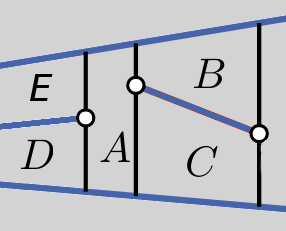
\includegraphics[width=0.3\textwidth]{neighbors}
	\caption{Ein Trapez mit vier Nachbarn}
	\label{fig:neighbors}
\end{figure}
In Abbildung \ref{fig:neighbors} ist ein Trapez $A$ gezeigt, welches vier Nachbarn hat. Wir haben uns dazu entschlossen, die Nachbarn diese entsprechend der Himmelsrichtungen zu bezeichnen. Somit ist $B$ der nordöstliche , C der südöstliche, D der südwestliche und E der nordwestliche Nachbar.

\subsection{Trapezzerlegung und Suchstruktur}

Als Datenstruktur für die Trapezzerlegung \T haben wir die Python-Klasse \texttt{set} verwendet, da diese zahlreiche Methoden für mathematische Mengen zur Verfügung stellt. \T enthält somit lediglich die Menge aller zur Trapezzerlegung gehörenden Trapeze.\\
Für die Suchstruktur \D haben wir die neue Klasse \texttt{Tree} entworfen. Ein Objekt dieser Klasse hat zum einen ein Attribut, welches den 'Inhalt' des Knotens speichert. Dabei kann es sich um eine Strecke, einen Punkt oder ein Trapez handeln. Zum anderen speichert es einen Links- und einen Rechtsverweis auf sein linkes bzw. rechtes Kind. Soll für einen Anfragepunkt $\rho$ ermittelt werden, in welchem Trapez dieser liegt, wird die Suchstruktur beginnend mit dem Wurzelknoten hinabgestiegen und dabei bei Punkten ermittelt, ob $\rho$ links oder rechts davon liegt, und bei Strecken, ob $\rho$ darüber oder darunter liegt. Entsprechend wird dann rekursiv mit dem linken bzw. rechten Kindknoten fortgefahren. Wird ein Blattknoten und damit ein Trapez erreicht, wird dieses als das den Punkt $\rho$ beinhaltendes Trapez als Antwort zurückgeliefert.


\section{Programmnutzung}
Bei den Programmen zur Trapezzerlegung und Pfadsuche handelt es sich um Python3-Programme. Daher muss auf der Zielplattform eine Python3-Runtime installiert sein, das ältere Python2 wird nicht unterstützt. Darüber hinaus weisen die Programme keine externen Abhängigkeiten (etwa zu Drittbibliotheken) auf.

\paragraph{Trapezzerlegung} Die Trapezzerlegung wird in der Datei \texttt{trapezoid\_decomposition.py} realisiert. Die Syntax zum Programmaufruf lautet

\begin{quotation}
	\texttt{python3 trapezoid\_decomposition.py [-h] [-i] [-d] [-l] in\_file out\_file}
\end{quotation}

\begin{tabular}{|l|c|l|}
	\hline
	Parameter & erforderlich & Bedeutung \\
	\hline
	in\_file & * & \pbox{10cm}{Der Pfad zur Eingabedatei, in der die Punkte, Strecken und Abfragepunkte gespeichert sind} \\
	out\_file & * & Der Pfad zur Datei, in die die Ausgabe geschrieben wird \\
	h & & Hilfe zum Programmaufruf anzeigen \\
	i & & Die Eingabedaten (\textbf{i}nput) visualisieren \\
	d & & Die Zerlegung (\textbf{d}ecomposition) visualisieren \\
	l & & Lokalisierungsergebnisse (\textbf{l}ocalization) visualisieren \\
	\hline
\end{tabular}

Die Visualisierungsoptionen können alle im selben Aufruf genutzt werden.

\paragraph{Pfadsuche} Die Pfadsuche mittels Trapezzerlegung wird in der Datei \texttt{path\_finding.py} realisiert. Die Syntax zum Programmaufruf lautet

\begin{quotation}
	\texttt{python3 path\_finding.py [-h] [-d] [-r] [-p] in\_file out\_file}
\end{quotation}

\begin{tabular}{|l|c|l|}
	\hline
	Parameter & erforderlich & Bedeutung \\
	\hline
	in\_file & * & \pbox{10cm}{Der Pfad zur Eingabedatei, in der die Hindernisse und Start- sowie End-punkte der zu findenden Pfade gespeichert sind} \\
	out\_file & * & \pbox{10cm}{Der Pfad zur Datei, in die die gefundenen Pfade geschrieben werden} \\
	h & & Hilfe zum Programmaufruf anzeigen \\
	d & & \pbox{10cm}{Die Trapezzerlegung (\textbf{d}ecomposition) der Eingabedaten visualisieren, nachdem die Hindernis-Trapeze entfernt wurden} \\
	r & & Die \textbf{R}oad-map visualisieren \\
	p & & Die gefundenen Pfade (\textbf{p}aths) visualisieren \\
	\hline
\end{tabular}

Die Visualisierungsoptionen können alle im selben Aufruf genutzt werden.

\section{Kram}

\begin{itemize}
\item Erstes Trapez finden (0.99p + 0.01q)
\item Wie werden mehrere gefundene Trapeze unterteilt?
\item Wie Trapzen Facetten zugeteilt werden
\item Gruppen der Punkte anhand der Facetten
\item Wie werden die Nachbarn zugeordnet (Himmelsrichtungen?)
\end{itemize}

\end{document}










